%%%%%%%%%%%%%%%%%%%%%%%%%%%%%%%%%%%%%%%%%%%%%%%%%%%%%%%%%%%%%%%%%%% 
%                                                                 %
%                            CHAPTER THREE - Intelligent Agent Construction - Version 1                        %
%                                                                 %
%%%%%%%%%%%%%%%%%%%%%%%%%%%%%%%%%%%%%%%%%%%%%%%%%%%%%%%%%%%%%%%%%%% 
 
%\chapter{Intelligent Agent Construction}
%
%This chapter describes an initial attempt at creating an intelligent agent based on shallow techniques.

\chapter{Version 1 -- A Shallow Agent}\blfootnote{This work previously appeared as: \bibentry{johnson2015cfeagent}} 

This chapter describes the approach taken to develop an intelligent agent using strictly shallow natural language processing (NLP)  techniques \cite{martin_2000_speech_ch23}.  It should be emphasized here that these algorithms are simplistic, some of which exploit structural patterns of the exam questions while others rely on bag of words techniques, in order to observe how well the agent performs with relatively little intelligence.  Performance measurements indicate this agent performs surprisingly well.  Some of the algorithms based on question structure, for example, reveal strong correlations with correct answers, as will be discussed in detail below, although the agent does not perform at a passing level.  Also, the agent provides very little justification for its answers, and thus, there is still ample motivation for a more sophisticated approach.

%\subsection{Resource Procurement and Customization}
\section{Resource Procurement and Customization}

The first phase of this project after downloading the study package was to convert its contents to a form that could be processed by an automated system.  The content in the package include the CFE Manual in pdf format, practice questions embedded within study package software, and a practice exam, also consisting of questions embedded within custom software.  It was necessary to convert each of these components into text-formatted documents for the CFE Agent.

The first of these components, the CFE Manual, is a 2,500 page pdf document that serves as the principal resource upon which all of the exam questions are based.  Conversion of this document involved an extensive amount of work for two reasons:  First, the pdf document itself was password protected, rendering most pdf conversion programs useless.  And second, the few software packages that \textit{were} capable of bypassing the password protection produced intermittent errors in the generated text, inserting spaces randomly between the letters of words.  Given the large volume of content, a program employing various parsing techniques was written to sequentially walk through the text, detect errors, make corrections automatically based on certain rules, or prompt for correction if an error was detected but manner of correction was uncertain.  Although a significant amount of effort was expended to develop this technology, in the end, much of the document was edited manually.  

\begin{figure}
\centering
\vspace{2.0in}
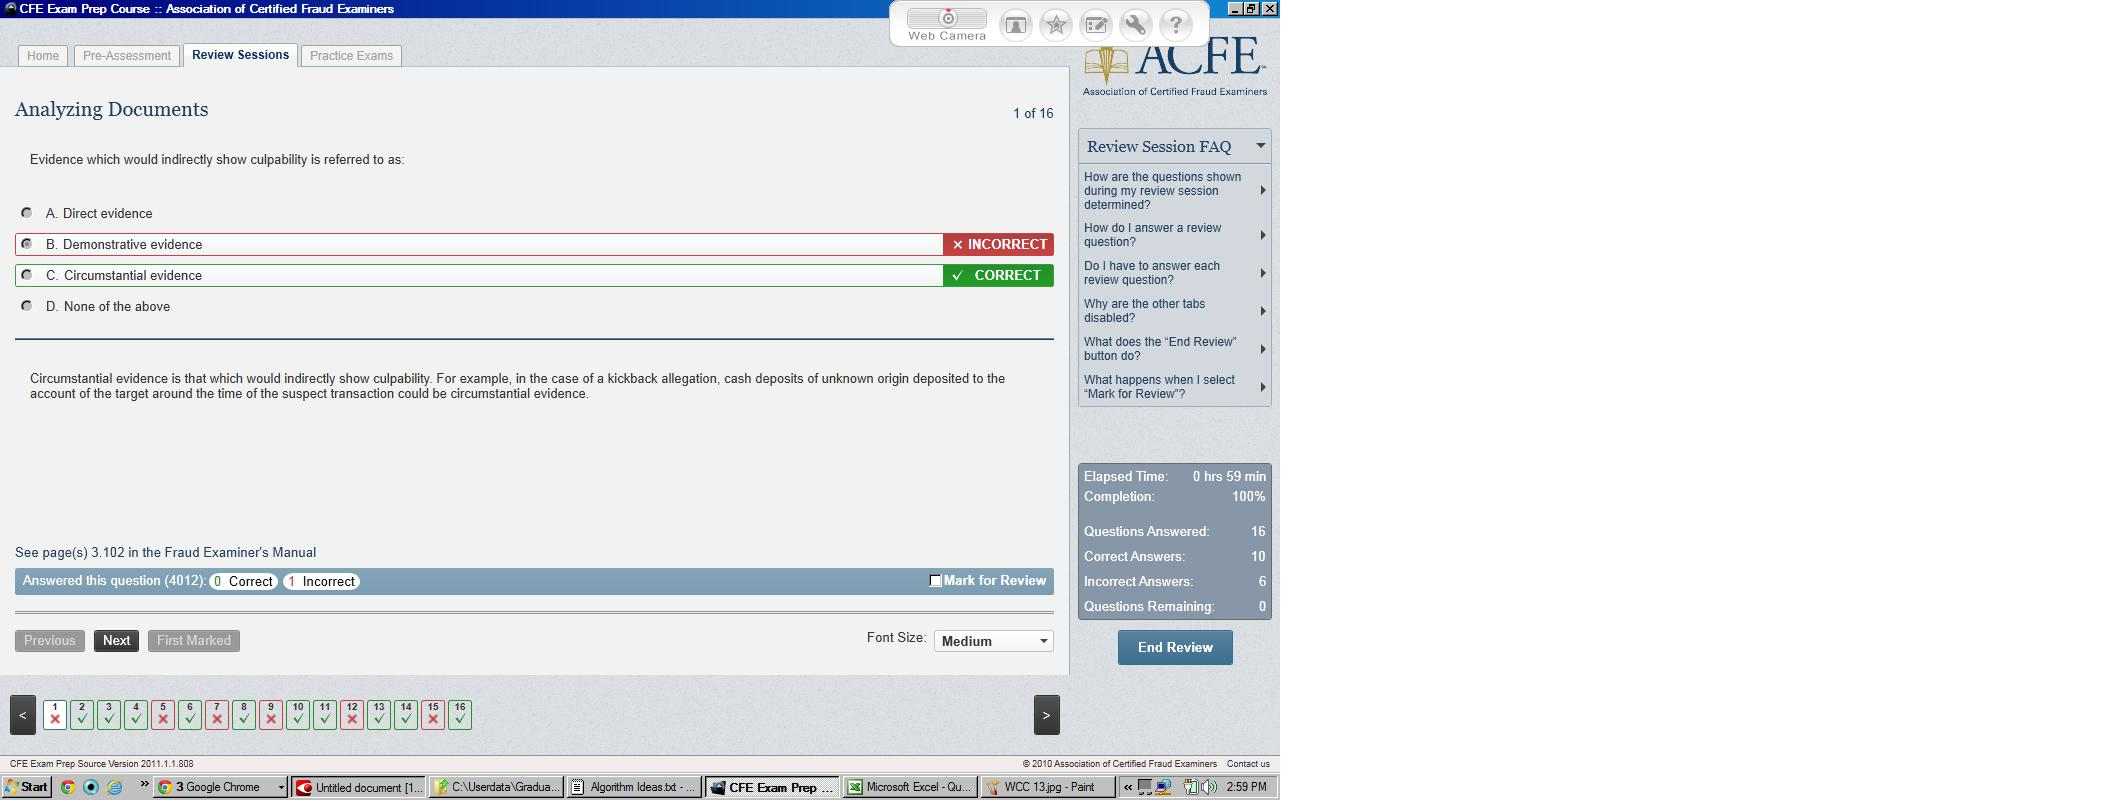
\includegraphics[width=200mm]{study_package_screen_shot.jpg}
\caption{Embedded Practice Question}
\label{fig:study_package_screen_shot}
\end{figure}

\begin{figure}
\centering
\vspace{2.0in}
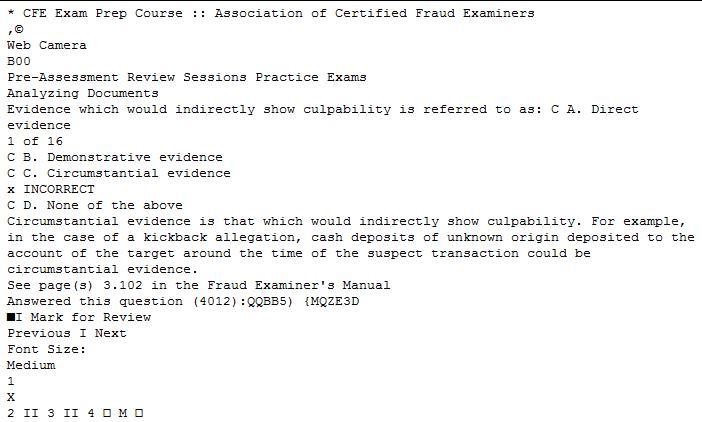
\includegraphics[scale=0.75]{study_package_unformatted_text.jpg}
\caption{Converted, Unscrubbed Practice Question}
\label{fig:study_package_unformatted_text}
\end{figure}

\begin{figure}
\centering
\vspace{2.0in}
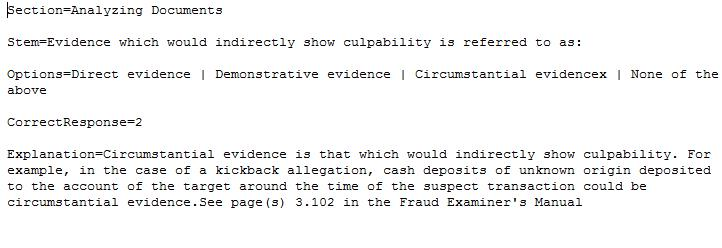
\includegraphics[scale=0.75]{study_package_formatted_text.jpg}
\caption{Scrubbed Practice Question}
\label{fig:study_package_formatted_text}
\end{figure}

The other main component of the prep package is the database of 1,500 questions embedded in the study package software.  The extraction of these questions from the software was an involved, multi-step process.  First, a screenshot file, as shown in Figure~\ref{fig:study_package_screen_shot},  was created for each question.  Second, optical character recognition (OCR) software was used to convert the graphic screen shot files into text files, as shown in Figure~\ref{fig:study_package_unformatted_text}.  Unfortunately, the important data needed for each question was intermingled among nonsensical overhead text in each of these text files.  So, a custom program was created to parse these text files, remove the unnecessary data, and decompose each question into its component parts --- topic, question stem, options, correct answer, and explanation --- as shown in Figure~\ref{fig:study_package_formatted_text}.  Finally, these files were manually reviewed and edited to ensure proper format for the agent.  The product of this process was a collection of 1,500 text files, one for each practice exam question, and each containing name-value pairs for the relevant question fields named above.




%\subsection{CFE Agent Design}
\section{CFE Agent Design}

The CFE Agent is an object-oriented program written in Java.  It takes as input a collection of question files and produces as output a sequence of answers which are, in turn, compared against the corresponding correct answers in order to calculate a score.  There are five principal elements to the design of the CFE Agent --- the CFE manual, the question profile, the algorithm set, algorithm profile data, and the algorithm-selection algorithm.

%\subsubsection{Question Profile}
\subsection{Question Profile}

After having reviewed the entire database of questions in the study package, it was determined that there are certain characteristics certain questions share in common.  This was thought to be a natural way of partitioning the questions according to a crude ontology each class of which could serve as a means for optimizing an algorithm for the questions of that class.  For example, one of the most obvious of these characteristics is whether the question is a true-false question or a multiple-choice question.  And if the question is true-false, does it include any of the following terms:  ``always'', ``never'', ``must'', or ``only''?  On the other hand, if a question is multiple choice, is its last option, ``All of the above''?  Some other criteria discovered that are worth noting are whether the question includes options with more than four words in it, whether the question contains the word ``except'', and whether the question's last option is ``None of the above''.

%\subsubsection{Algorithm Set}
\subsection{Algorithm Set}

Various algorithms were developed and incorporated into the model.  The system currently employs nine custom algorithms that utilize natural language processing, information retrieval, and general test-taking techniques.  Descriptions of a few example algorithms are given below:

\subsubsection{Max Joint Probability Algorithm}

This algorithm considers only the possible answers, treating each as a sequence of words whose joint probability is to be calculated.  It calculates this joint probability for each option by finding the probability of each word among the words of the manual section from which the question was drawn (indicated by topic) and by applying the simplifying assumption of independence between words.  The joint probability, then, is simply calculated as the product of the probabilities of the individual words of the option, normalized for the number of words (so that short answers are not over-weighted).  The algorithm selects the option with maximum joint probability.

\subsubsection{Max Frequency Algorithm}

The Max Frequency Algorithm simply counts up the total number of times each answer option is encountered in the manual section from which the question was drawn and selects the option whose tally is the largest.  Unlike the Max Joint Probability Algorithm, the frequencies are based on occurrences of entire phrases, not on the counts of individual words within them.

\subsubsection{False Select}

This algorithm applies only to true-false questions, simply selecting false, always.  Remarkably, this algorithm proved extremely effective for such questions that have ``must'', ``always'', ``only'', or ``never'' in the stem, achieving an astonishing 78.7\% accuracy rate on this class of questions.  The remarkable success of such a simple algorithm is an indication of the effectiveness of gaming strategies on certain questions, but also an indication of weaknesses in the way certain questions on this exam are designed.

\subsection{Algorithm Profile Data}

The algorithm profile data is a table showing accuracy each algorithm on each question question profile, tabulated from running every algorithm on every question in a training set of 1,297 question selected from the battery of 1,500 questions.  For each of these questions, a profiler component performed the following steps:  First, determine the question profile.  Second, execute each algorithm on the question, recording whether each algorithm produced the correct answer.  Finally, summarize the results.  A portion of this summary data is shown in Figure~\ref{fig:profile_data_training_set}

\begin{figure}
\centering
\vspace{2.0in}
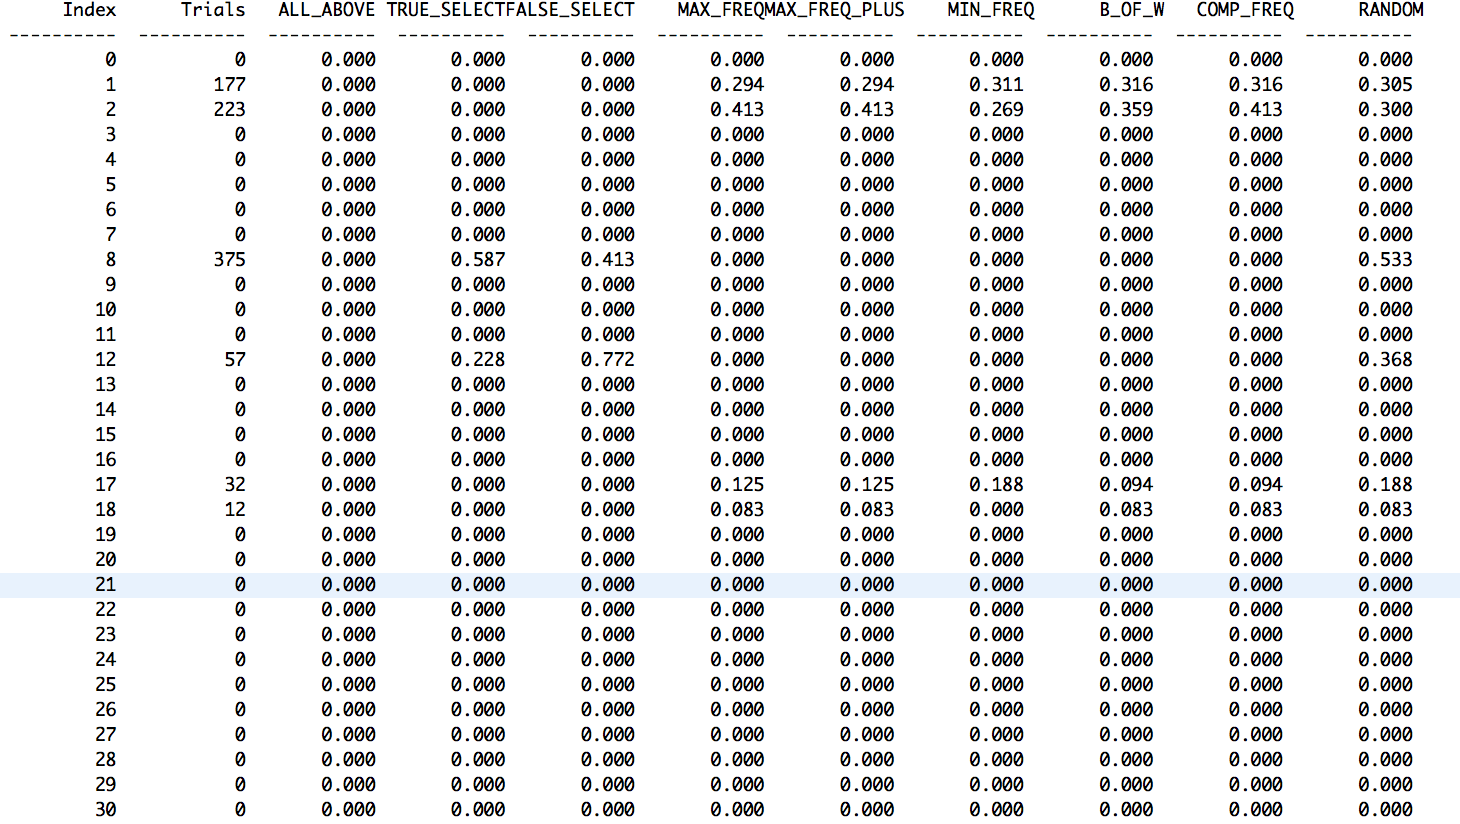
\includegraphics[scale=0.25]{profile_data_training_set.png}
\caption{Training Set Profile Data}
\label{fig:profile_data_training_set}
\end{figure}

%\subsubsection{The Selection Algorithm}
\subsection{The Selection Algorithm}

The selection algorithm is the procedure for selecting the proper algorithm to apply to a given question.  It is based on the algorithm profile data described above.  For a given question in the 203-question test set, the CFE Agent chooses the algorithm with the highest accuracy rate for questions in the training set with the same profile.

%\subsection{CFE Agent Demo}
\section{CFE Agent Demo}

This section outlines a walkthrough of the execution of the CFE Agent for a very short exam, consisting of only four questions.  Despite its short length, it should provide a good idea of the basic mechanics of the agent.  

Figure~\ref{fig:cfe_agent_startup} shows the startup of the agent.  The name of a configuration file is passed in as a command line parameter to the program.  This file provides a number of settings for the execution environment, including the mode (interactive vs. batch), the name of the exam file, and log detail level.  In this demo, the agent is executing with full detail so that it is easier to understand what is happening under the covers for each question.

The detail logging shows that one of the first things the CFE Agent does when it starts up is construct an internal representation of the CFE Manual.  This internal representation is in the form of a graph, each of whose nodes represents a section of the document.  More specifically, the graph is a tree whose root node represents the entire manual, which in turn possesses links to child nodes each representing one of the four main sections of the manual (Financial Transactions and Fraud Schemes, Law, Investigation, and Fraud Prevention and Deterrence) each of which in turn possesses child nodes representing sub-sections to those sections, and so on.  Each node stores information about the section it represents in addition to the text itself, including a hash table for word counts, sub-subheadings, et cetera.  This information facilitates the text analytic computations the agent performs as it answers questions on the exam.  It should be noted that much of the basis of this tree data structure is based on the items listed in the manual’s table of contents, and for even finer-grained detail nodes, on text features within the corpus itself.  (That is, lines of text consisting of all capital letters terminating in carriage return generally denote a sub-section of text).  Finally, in addition to the tree data structure, the internal representation of the manual includes additional data structures mapping the text of the manual for optimizing access to particular manual subsections.

\begin{figure}
\centering
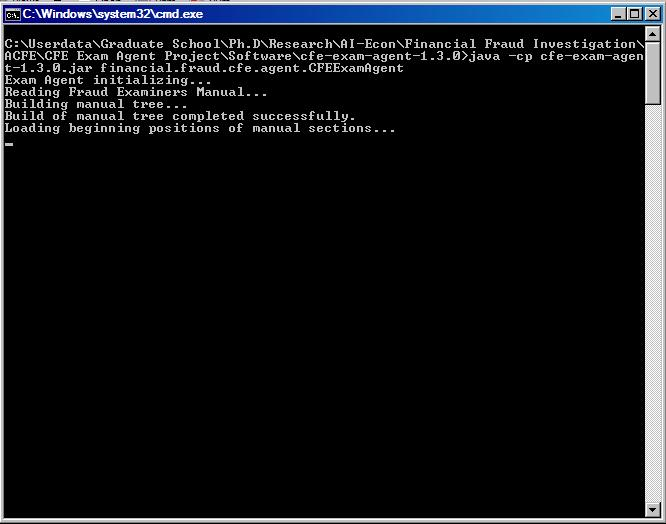
\includegraphics[scale=0.75]{screen_shot_1.jpg}
\caption{CFE Agent Startup}
\label{fig:cfe_agent_startup}
\end{figure}


In Figure~\ref{fig:cfe_agent_startup_completed}, the screen shows the completion of the startup sequence of the CFE Agent.  First, the CFE Agent gives a line-by-line report showing the nodes loaded into the tree data structure.  Then, it shows some additional configuration information showing the exam file, execution mode, and runtime status.  At this point, the CFE Agent is ready to begin the exam.

\begin{figure}
\centering
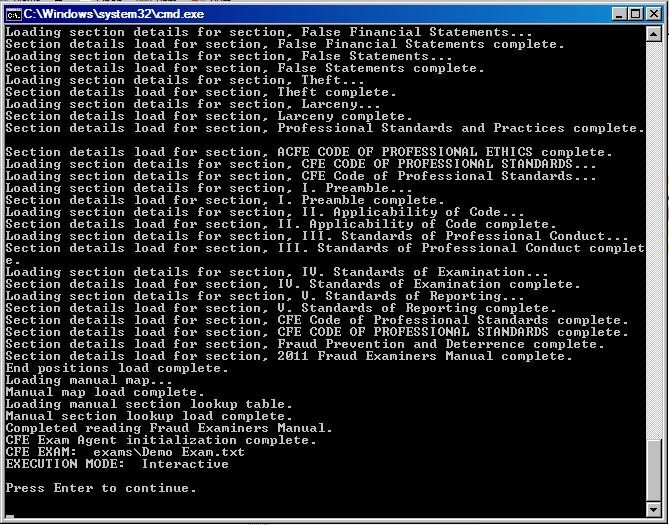
\includegraphics[scale=0.75]{screen_shot_2.jpg}
\caption{CFE Agent Startup Completed}
\label{fig:cfe_agent_startup_completed}
\end{figure}

In Figure~\ref{fig:first_question}, the first question of the exam is shown along with four possible answers.  After the user presses return, the CFE Agent selects the optimal algorithm for that particular question and executes it.  

\begin{figure}
\centering
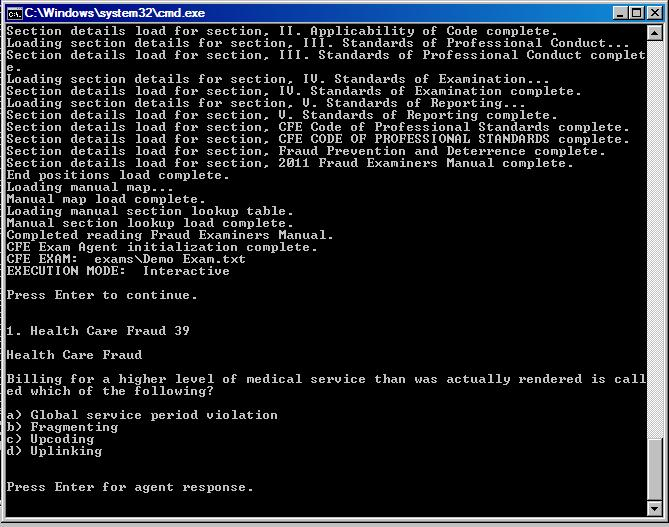
\includegraphics[scale=0.75]{screen_shot_3.jpg}
\caption{First Question}
\label{fig:first_question}
\end{figure}

Figure~\ref{fig:first_question_completed} shows log detail for the CFE Agent as it attempts to choose the correct answer for the first question.  First, as described in the discussion of the question profile, the agent makes an assignment to a question profile category based on some key features of the question, (whether it's a true-false question, a question at least one of whose options contains more than 4 words, et cetera).  Once it assesses the question profile, it chooses an algorithm which based on prior experience exhibits maximum accuracy on questions having the same profile.  For this question, the profile assignment is category 2, meaning the question has been categorized as a ``definition'' question – essentially one which attempts to test for knowledge of domain-specific vocabulary.  The experience data of the Agent indicates the best performing algorithm is the Max Frequency algorithm, which when applied for this question results in the selection of choice c, the correct answer.

\begin{figure}
\centering
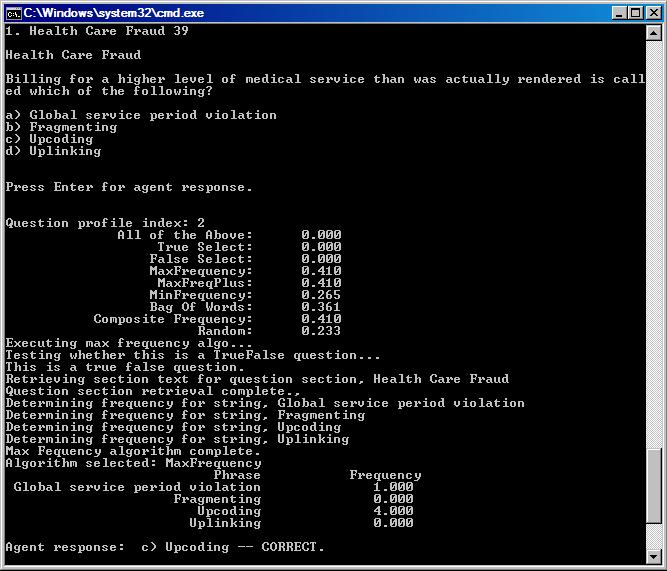
\includegraphics[scale=0.75]{screen_shot_4.jpg}
\caption{First Question Completed}
\label{fig:first_question_completed}
\end{figure}

Figure~\ref{fig:second_question} shows the CFE Agent answer the second question.  This question appears to be similar to the first in that it also earns a category assignment of 2, meaning it is another ``definition'' question.  By the same experience-based reasoning as in the first question, the agent applies the Max Frequency algorithm and selects answer a, the correct answer.

\begin{figure}
\centering
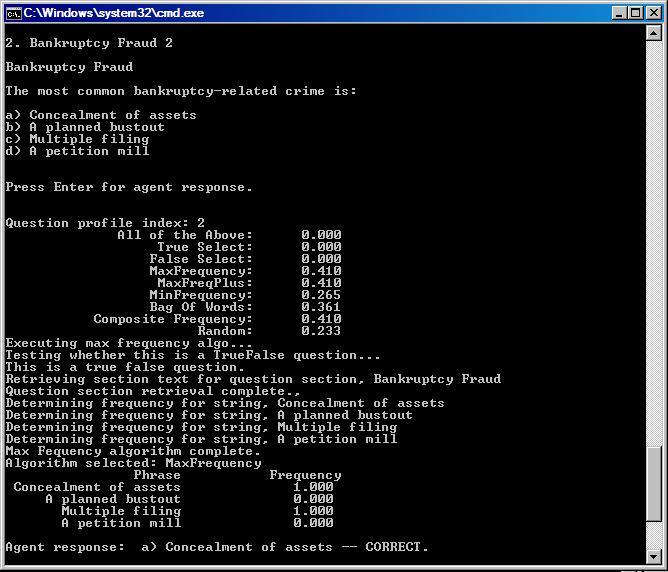
\includegraphics[scale=0.75]{screen_shot_5.jpg}
\caption{Second Question}
\label{fig:second_question}
\end{figure}

Figure~\ref{fig:third_question} shows an attempt at the third question.  However, this time the agent is not successful at choosing the right answer.  Again, it assigns this question to the same category as the two prior questions and uses the same Max Frequency algorithm, but it is led astray by the fact that the fourth option, ``cost'' is a common word whose frequency in the section corpus is over-weighted relative to the other options for this question.  This is an example where the current level of sophistication of the agent is insufficient to correctly answer questions one of the options may consists of a word or phrase that might be over-represented in the corpus.  Further work will need to be done to develop the natural language processing algorithm to compensate for this over-weighting, while preserving its relative success on other questions in the same category.

\begin{figure}
\centering
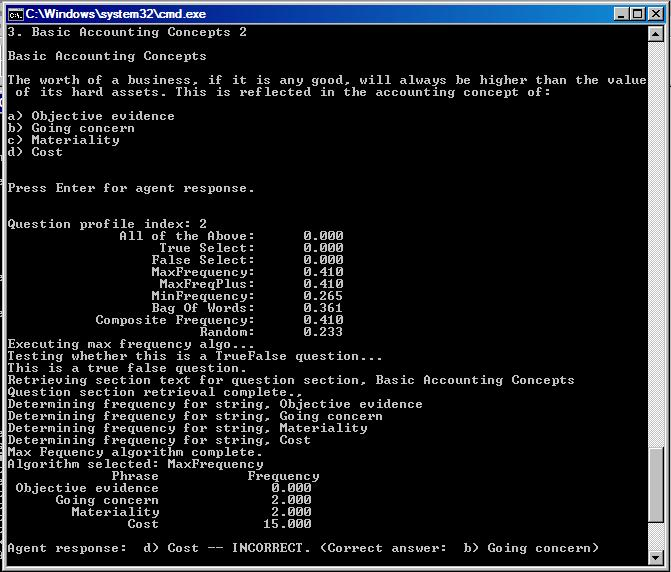
\includegraphics[scale=0.75]{screen_shot_6.jpg}
\caption{Third Question}
\label{fig:third_question}
\end{figure}

Figure~\ref{fig:final_question_and_termination} shows the final question, which is one of a different type --- an ``All of the Above'' question.  Here, the CFE Agent chooses an algorithm appropriately called ``All of the Above'' because it simply selects ``All of the Above'' whenever its an option.  (As shown in the data table, this algorithm has a remarkable 86\% success rate, lending one to question certain aspects of the CFE Exam’s design, as mentioned earlier.)  The agent applies this algorithm and gets the answer correct.  Finally, the agent terminates.

\begin{figure}
\centering
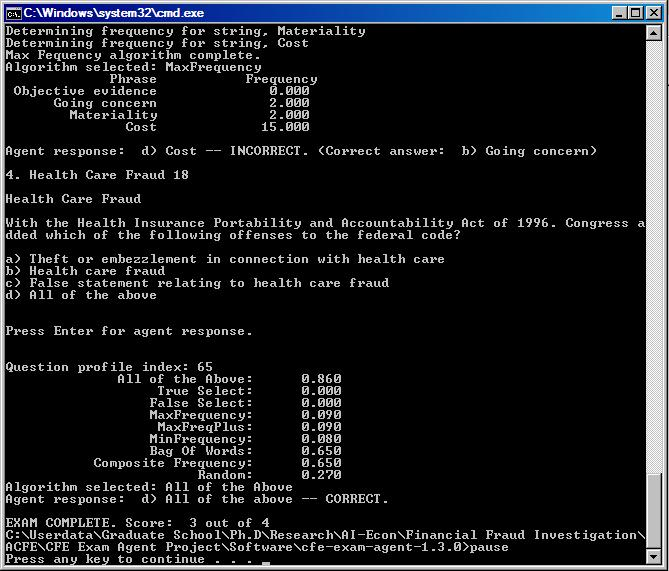
\includegraphics[scale=0.75]{screen_shot_7.jpg}
\caption{Final Question and Termination}
\label{fig:final_question_and_termination}
\end{figure}


%\subsection{CFE Agent Results - A Good Start}
\section{CFE Agent Results - A Good Start}

A detailed look at the performance of the agent on the entire battery of 1,500 questions, assuming the agent employs the most accurate algorithm for each question, given its profile, shows the agent demonstrates promising, statistically significant performance.  Consider the question of whether the agent actually performed any better than random guessing.  For true-false questions, random guessing would be expected to yield an accuracy rate on the of approximately 50\%.  (Given there are a relatively large number of true-false questions (506), it is reasonable to assume the experimental accuracy rate should be very close to this theoretical value.)  Likewise, for multiple-choice questions with four options, random guessing should yield an accuracy rate of approximately 25\%.  (Again, for the same reason as for true-false questions, the experimental accuracy should be close to the theoretical expected value.)  However, the empirical data shown in Figure~\ref{fig:results_for_true_false_questions} and Figure~\ref{fig:results_for_multiple_choice_questions} indicates that for true-false questions, the observed accuracy rate is over 58\% on this training set, giving a z-score of over 3.729 (the z-score for a p-value of 1\% is 2.575), and that for multiple-choice questions, the accuracy rate is just over 47.8\%, giving a z-score of 16.67.  For both classes of questions, then, the null hypothesis of performance consistent with random guessing is rejected by a large margin at the 99\% significance level.  


\begin{figure}
\centering
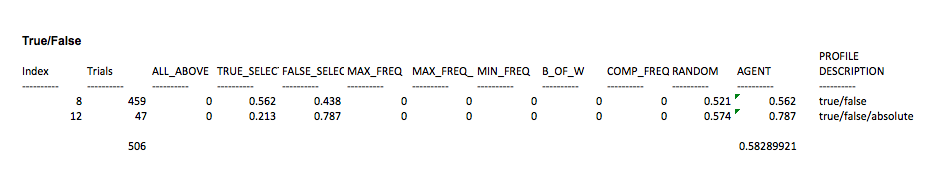
\includegraphics[width=130mm]{true_false_results_1500.png}
\caption{Results for True-False Questions}
\label{fig:results_for_true_false_questions}
\end{figure}

\begin{figure}
\centering
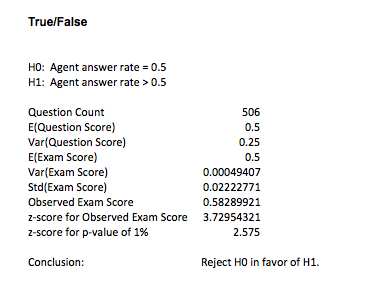
\includegraphics[scale=0.75]{true_false_hypothesis_test_1500.png}
\caption{Hypothesis Test for True-False Questions}
\label{fig:hypothesis_test_for_true_false_questions}
\end{figure}

\begin{figure}
\centering
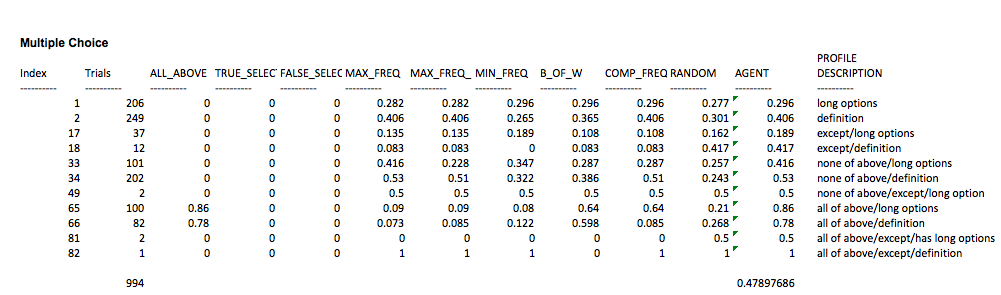
\includegraphics[width=130mm]{multiple_choice_results_1500.png}
\caption{Results for Multiple-Choice Questions}
\label{fig:results_for_multiple_choice_questions}
\end{figure}

\begin{figure}
\centering
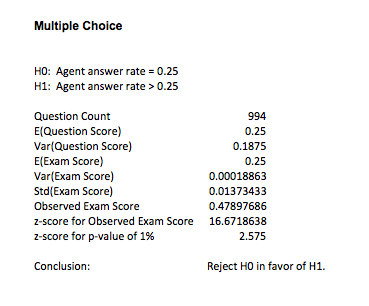
\includegraphics[scale=0.75]{multiple_choice_hypothesis_test_1500.png}
\caption{Hypothesis Test for Multiple-Choice Questions}
\label{fig:hypothesis_test_for_multiple_choice_questions}
\end{figure}
 

The above analysis covers the entire battery of 1,500 questions.  However, in developing our agent, this battery was broken into two subsets - a training set consisting of 1,300 questions and a test set consisting of 200 questions.  The idea here is to utilize the training set to determine the optimum algorithm for each profile (that is, the one whose accuracy is highest), and then to apply that knowledge on the test set by applying the best algorithm for each question, based on its profile.  The process of breaking the collection of questions up into a training set and test set was done via a programmatic procedure that selected a random, proportionate selection of questions for each CFE-exam subtopic.  Figure~\ref{fig:version_1_training_set_results} shows the results for the training set are comparable to those for the 1,500-question battery, as should be expected.  Using this data, the CFE Agent was executed on the 200-question test set, where it answered 98 correct, or 49\%.  Although this is short of passing, it's an encouraging start, and provides a good baseline for subsequent versions of the agent.

\begin{figure}
\centering
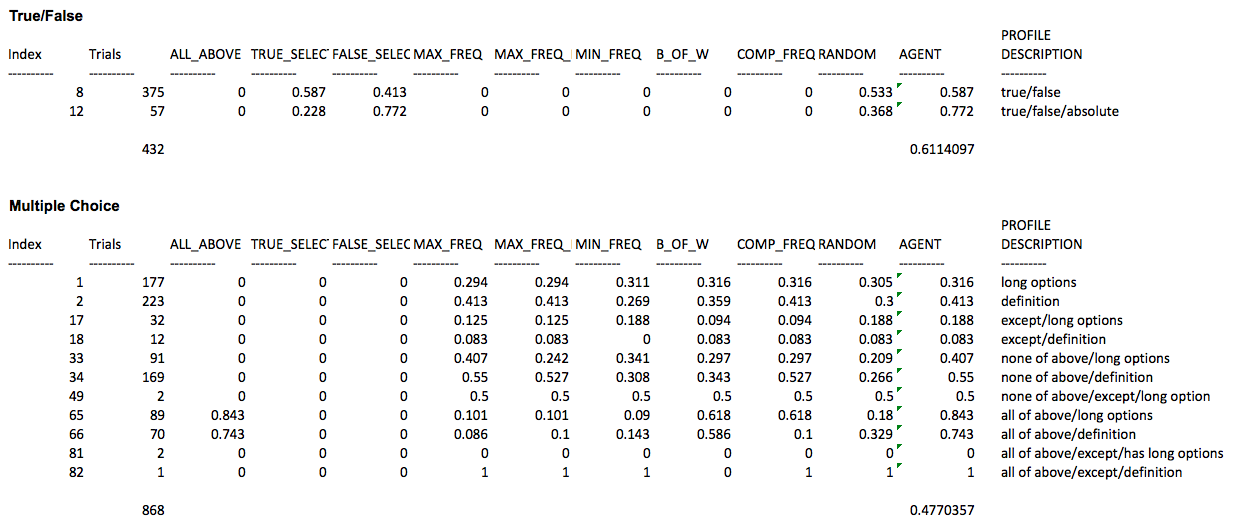
\includegraphics[width=130mm]{version_1_training_set_results.png}
\caption{Results for Multiple-Choice and True-False Questions on 1300-Question Training Set}
\label{fig:version_1_training_set_results}
\end{figure}

Finally, it should also be pointed out that during development of later versions of the agent, it was noticed that an important question feature had been overlooked in the original analysis -- the notion of a ``not'' question.  An example of a not question is:  ``Which of the following is NOT one of the major standards of generally accepted accounting principles?''.  It was found to be necessary to break out questions of this variety from other questions that were otherwise of the same type, but did not include the ``NOT'' term.  Thus, the analysis was completed once more on the training set, showing the following results in Figure~\ref{fig:version_1_training_set_results_not}.  It should be noted from this table, for example, that among the 223 questions formerly  categorized as ``definition'' questions, 40 are now categorized as ``definition/not'' questions.  The same phenomenon occurred for other categories, as well.  This last table provides the ultimate baseline against which we can make comparisons of effectiveness of algorithms going forward.

\begin{figure}
\centering
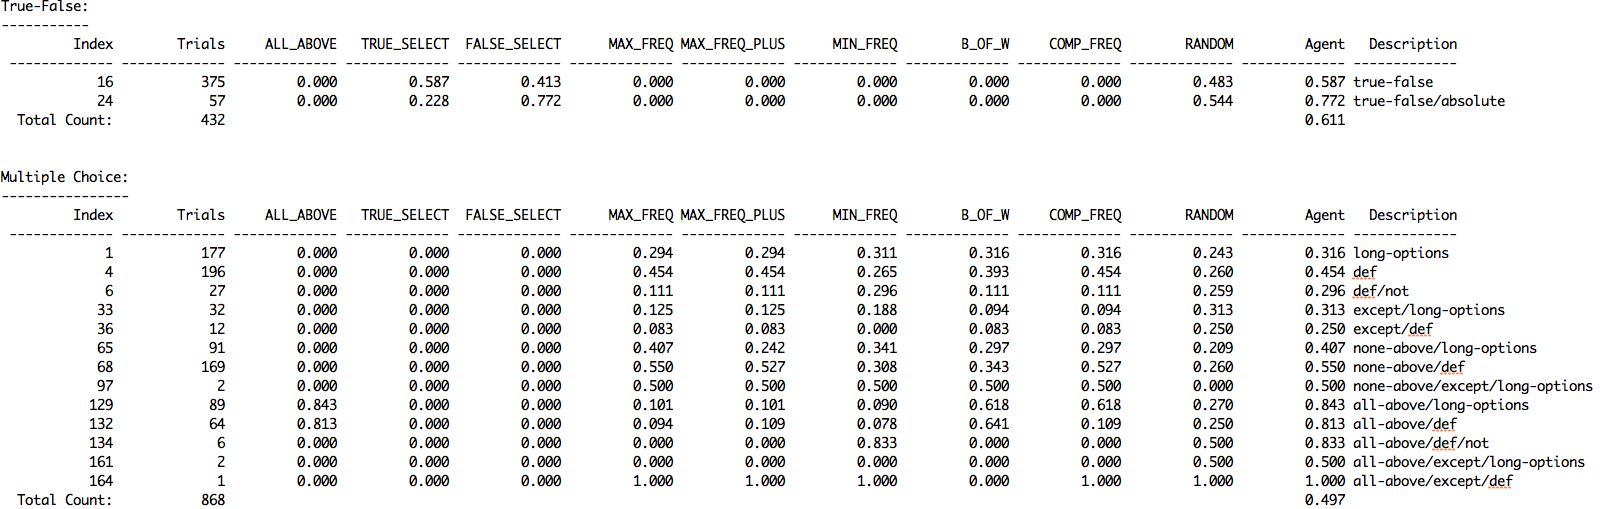
\includegraphics[width=130mm]{version_1_training_set_results_not.png}
\caption{Training Set Results with NOT Feature Breakout}
\label{fig:version_1_training_set_results_not}
\end{figure}



